Describe requirements to meet detector goals

\subsection{LBNF detector}
This section to provide context and illustrate which aspects need testing at the CERN prototype

(Probably can take text from CDR once it's more developed)

\subsection{CERN prototype detector}

\subsubsection{Cryostat from David Montanari}
The Single Phase TPC test at CERN will use a membrane tank technology to contain the base design of 725 tons of LAr equivalent to about $520 m^3$. The design is based on a scaled up version of the LBNE 35 Ton Prototype and the Fermilab Short Baseline Near Detector. We propose that the cryostat be housed in the extension of the EHN1 Bat 887 at CERN, where the cryogenic system components will also be located. The cryostat will use a steel outer supporting structure with a metal liner inside to isolate the insulation volume, similar to the one of the dual phase detector prototype WA105 $1\times1\times3$ and to the Fermilab Short Baseline Near Detector. The support structure will rest on I-beams to allow for air circulation underneath to maintain the temperature within the allowable limits.
The scope of the EHN1 cryostat subsystem includes the design, procurement, fabrication, testing, delivery and oversight of a cryostat to contain the liquid argon and the TPC. This section describes a reference design, whose scope encompasses the following components:

\begin{itemize}
\item steel outer supporting structure,
\item main body of the membrane cryostat (sides and floor), 
\item top cap of the membrane cryostat.
\end{itemize}

A membrane cryostat design commonly used for liquefied natural gas (LNG) storage and transportation will be used. In this vessel a stainless steel membrane contains the liquid cryogen. The pressure loading of the liquid cryogen is transmitted through rigid foam insulation to the surrounding outer support structure, which provides external support. The membrane is corrugated to provide strain relief resulting from temperature related expansion and contraction. The vessel is completed with a top cap that uses the same technology.

Two membrane cryostat vendors are known: GTT (Gaztransport \& Technigaz) from France and IHI (Ishikawajima-Harima Heavy Industries) from Japan. Each one is technically capable of delivering a membrane cryostat that meets the design requirements for this detector. To provide clarity, only one vendor is represented in this document, GTT; this is for informational purposes only. Figure 1 shows a 3D model of the GTT membrane and insulation design.


\begin{figure}
\begin{center}
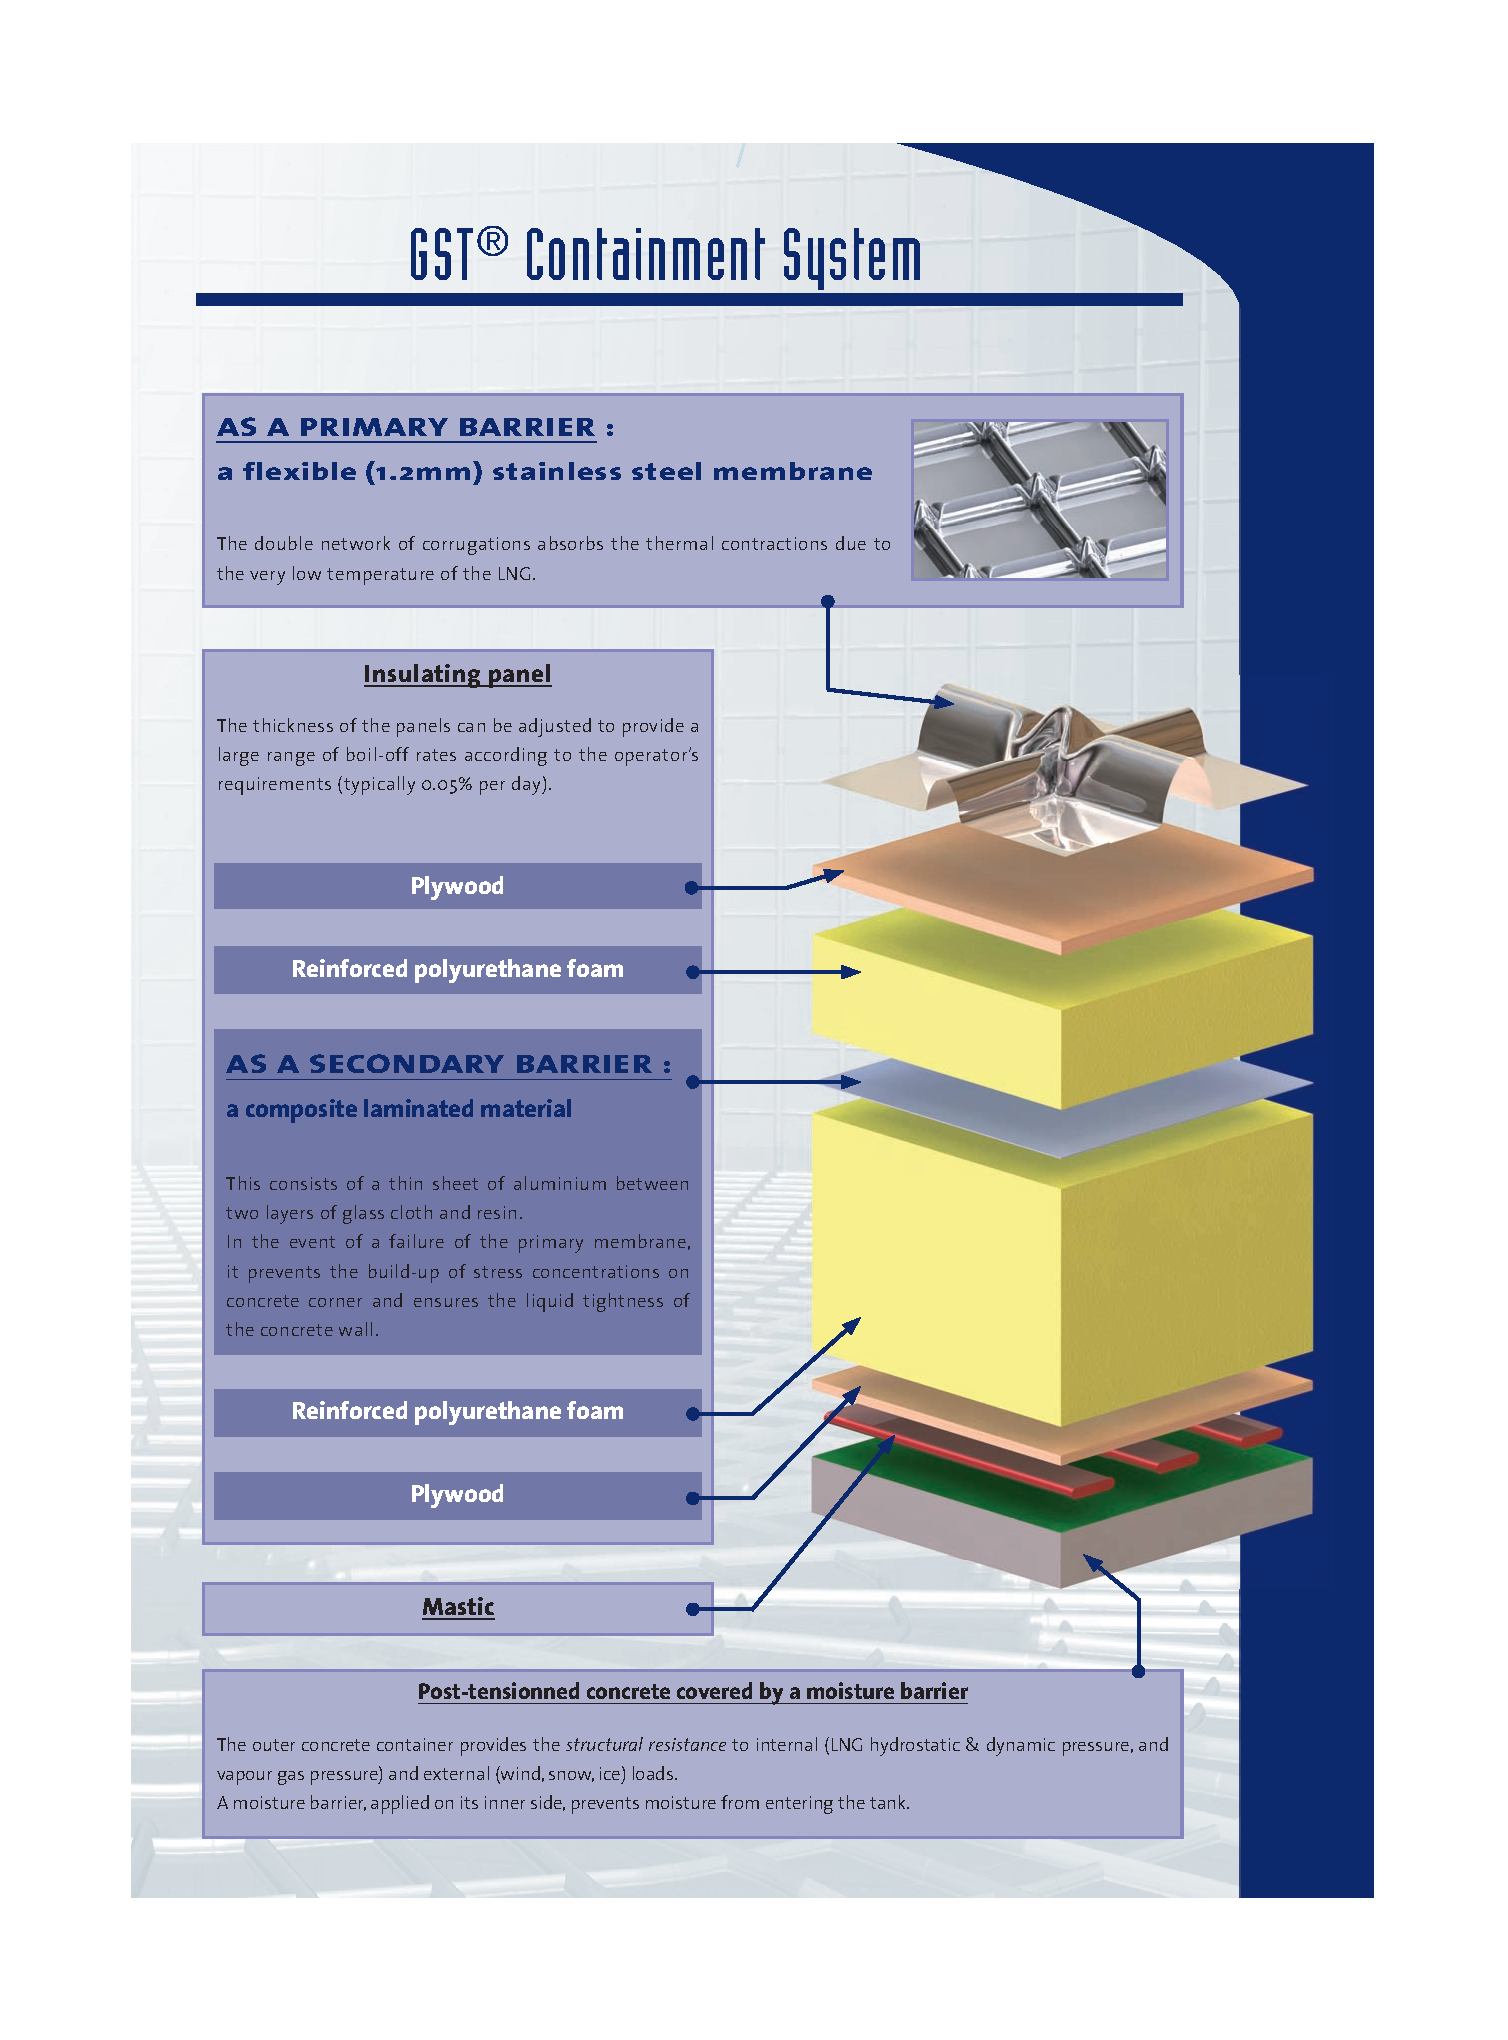
\includegraphics[width=.9\textwidth]{figures/membrane-exploded-view} % (figure 1)
\caption[Exploded view of the membrane cryostat technology]{\label{fig:lar-org} Exploded view of the membrane cryostat technology}
\end{center}
\end{figure}

The conceptual reference design for the Single Phase Test at CERN cryostat is a rectangular vessel measuring 9.5 m in length (parallel to the beam direction), 7.3 m in width, and 8.40 m in height; containing a total mass of 725 tons of liquid argon. Figure~\ref{fig:cryostat-views} shows side and end views of the cryostat respectively. Figure 3 shows a 3D view. To minimize the contamination from warm surfaces, during operation the temperature of all surfaces in the ullage shall be lower than 100 K. The top plate will contain two hatches to install the TPCs and enter the tank, a manhole and several penetrations for the cryogenic system and the detector.

\begin{figure}
\begin{center}
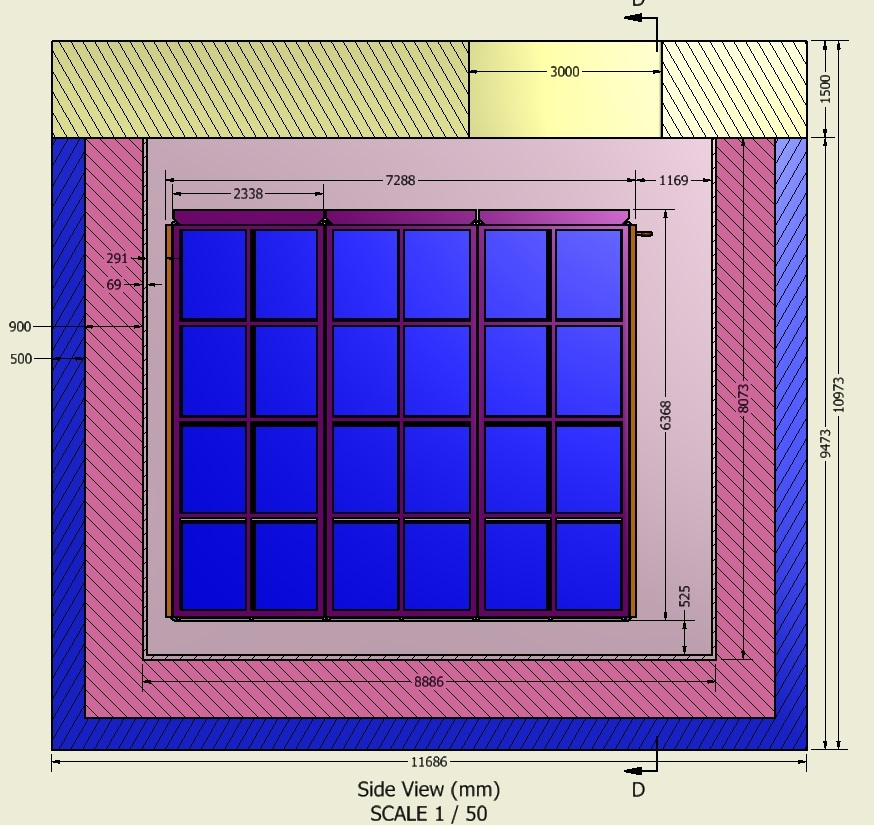
\includegraphics[width=.55\textwidth]{figures/cryostat-side-view} % (figure 2a)
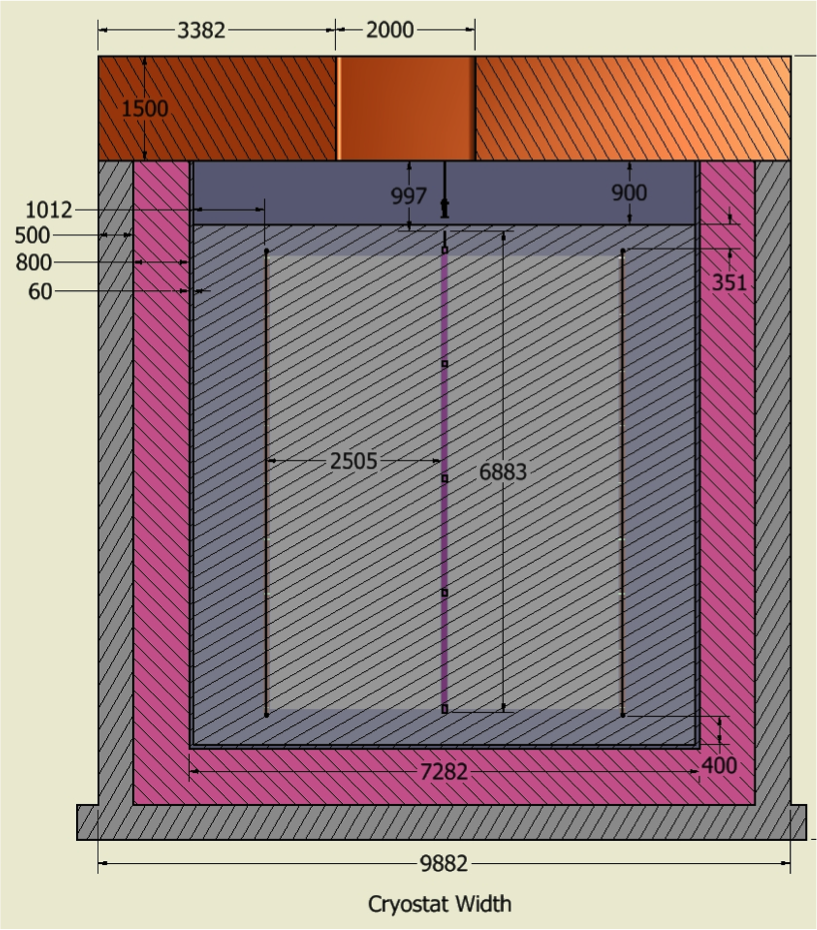
\includegraphics[width=.35\textwidth]{figures/cryostat-end-view}  %(figure 2b)
\caption[Views of cryostat]{\label{fig:cryostat-views} Side (left) and end (right) views of cryostat}
\end{center}
\end{figure}

\begin{figure}
\begin{center}
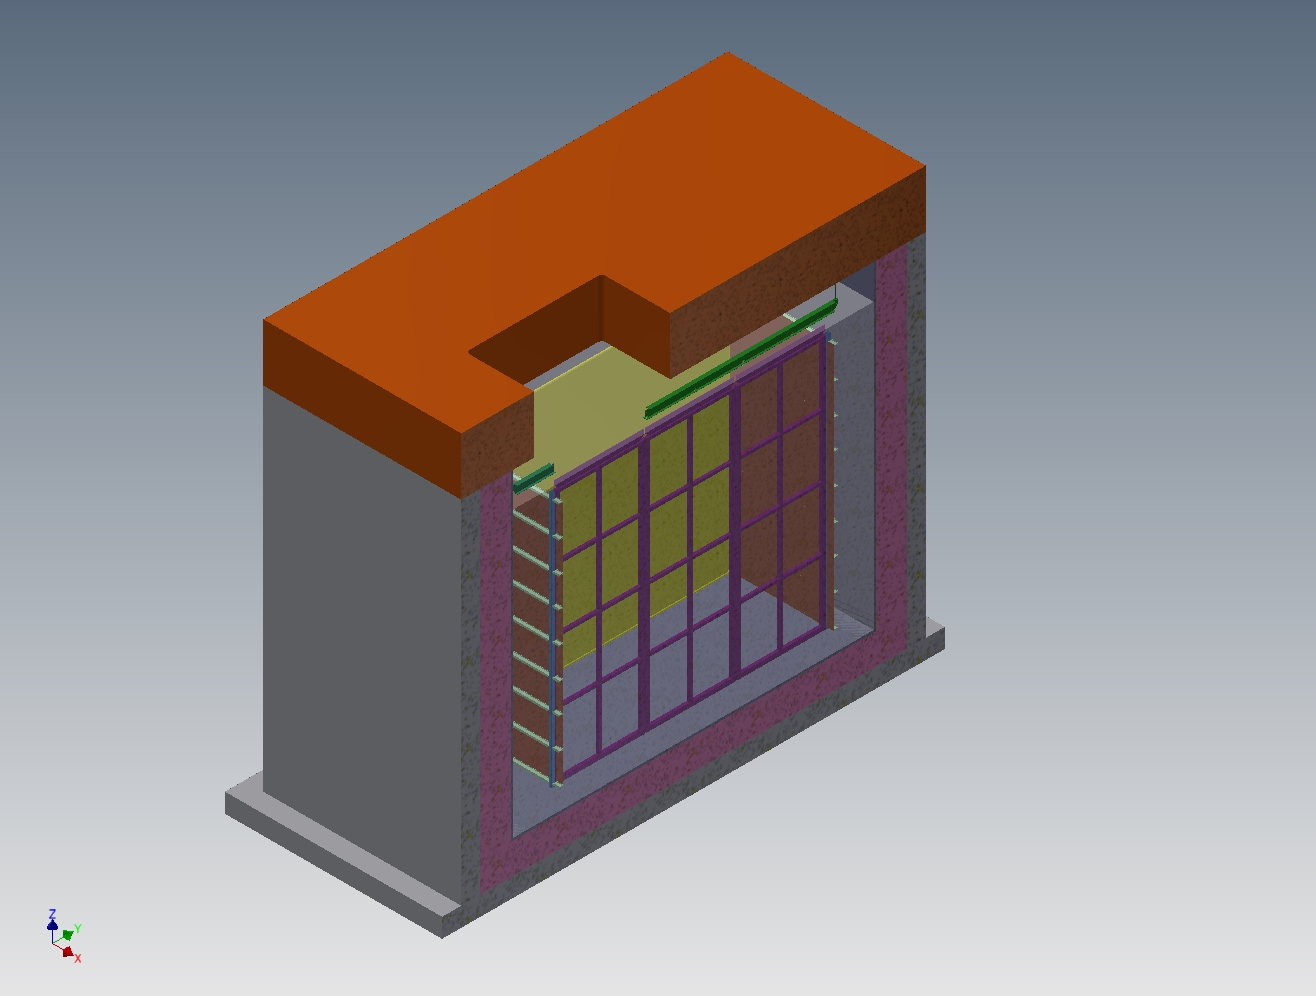
\includegraphics[width=.75\textwidth]{figures/cryostat-isometric-view} % (figure 3)
\caption[Isometric view of cryostat]{\label{fig:cryostat-views} Isometric view of the membrane cryostat}
\end{center}
\end{figure}

\textbf{Design Parameters (from David Montanari)}

This design is meant to test technical solutions that may be of interest for future needs of the Long Baseline Neutrino program. The use of a cold ullage (\textless 100 K) to lower the impurities in the gas region, and of a LAr pump outside the cryostat to minimize the effect of noise, vibration and microphonics to the TPC inside the LAr are Value Engineering studies for the Long Baseline program.

The design parameters for the TPC Test at CERN cryostat are listed in Table~\ref{tbl:cryogenics-design-parameters}.

\begin{table}[htpb]
\caption{Design requirements for the cryogenic system (has right values)}
\label{tbl:cryogenics-design-parameters}
\centering
\begin{tabular}{|p{.4\textwidth}|p{.5\textwidth}|}
\hline
\textbf{Design Parameter} & \textbf{Value} \\ \hline
Type of structure & Membrane cryostat \\ \hline
Membrane material    &  SS 304/304L, 316/316L or equivalent. 
Other materials upon approval.\\ \hline
 Outside reinforcement (support structure)  &  Steel enclosure with metal liner to isolate the outside from the insulation space, standing on legs to allow for air circulation underneath. \\ \hline
 Total cryostat volume  &  583 m3 \\ \hline
 Total LAr volume  &  520 m3 \\ \hline
LAr total mass   & 725,000 kg  \\ \hline
Minimum inner dimensions (flat plate to flat plate).   &  7.3 m (W) x 9.5 m (L) x 8.4 m (H) \\ \hline
Depth of LAr   &  7.5 m (0.9 m ullage, same as LBNF) \\ \hline
Primary membrane   &   1.2 mm thick SS 304L corrugated stainless steel\\ \hline
Secondary barrier system   &  0.07 mm thick aluminum between fiberglass cloth. Overall thickness 1 mm located between insulation layers.  \\ \hline
 Insulation  &  Polyurethane foam (0.8 m thick from preliminary calculations) \\ \hline
Maximum static heat leak   &  15 W/m2 \\ \hline
LAr temperature   & 88 +/- 1K  \\ \hline
Operating gas pressure   &  Positive pressure. Nominally 70 mbarg (~1 psig) \\ \hline
 Vaccuum  &  No vacuum \\ \hline
 Design pressure  &  350 mbarg (~5 psig) + LAr head (1,025 mbarg) \\ \hline
Design temperature   &  77 K (liquid nitrogen temperature for flexibility) \\ \hline
Temperature of all surfaces in the ullage during operation   &   \\ \hline
Leak tightness   & \textless 100 K  \\ \hline
Maximum noise/vibration/microphonics inside the cryostat   & LAr pump outside the cryostat  \\ \hline
Beam window   & In the center of the active volume. 
Precise location TBD.   \\ \hline
 Accessibility after operations  & Capability to empty the cryostat in 30 days and access it in 60 days after the end of operations. \\ \hline
  Lifetime / Thermal cycles &  Consistent with liquid argon program. TBD. \\ \hline
 \end{tabular}
\end{table}

\textbf{Insulation system and secondary membrane (from David Montanari)}

The membrane cryostat requires insulation applied to all internal surfaces of the outer support structure 
and roof in order to control the heat ingress and hence required refrigeration heat load. The maximum 
required static heat leak is $15 W/m^2$ for the floor and the sides and $20 W/m^2$ for the roof. 
Preliminary calculations show that it can be obtained using 0.8 m thick insulation panels. Given an 
average thermal conductivity coefficient for the insulation material of 0.0283 W/(m·K), the heat input 
from the surrounding steel is expected to be about 3.7 kW total. It assumes that the hatches are foam 
insulated as well. This is shown in Table~\ref{tbl:heat-load-calc}.

The insulation material is a solid reinforced polyurethane foam manufactured as composite panels. The 
panels get laid out in a grid with 3 cm gaps between them (that will be filled with fiberglass) and fixed 
onto anchor bolts anchored to the support structure. The composite panels contain the two layers of 
insulation with the secondary barrier in between. After positioning adjacent composite panels and filling 
the 3 cm gap, the secondary membrane is spliced together by epoxying an additional overlapping layer 
of secondary membrane over the joint. All seams are covered so that the secondary membrane is a 
continuous liner.

The secondary membrane is comprised of a thin aluminum sheet and fiberglass cloth. The fiberglass-
aluminum-fiberglass composite is very durable and flexible with an overall thickness of about 1 mm. The 
secondary membrane is placed within the insulation space. It surrounds the bottom and sides. In the 
unlikely event of an internal leak from the primary membrane of the cryostat into the insulation space, it 
will prevent the liquid cryogen from migrating all the way through to the steel support structure where it 
would degrade the insulation thermal performance and could possibly cause excessive thermal stress in 
the support structure. The liquid cryogen, in case of leakage through the inner (primary) membrane will 
escape to the insulation volume, which is purged with GAr at the rate of one volume exchange per day.

\begin{table}[htpb]
\caption{Heat load calculation for the membrane cryostat (insulation thickness = 0.8 m). (note to self: has right values)}
\label{tbl:heat-load-calc}
\centering
\begin{tabular}{|p{.15\textwidth}|p{.15\textwidth}|p{.15\textwidth}|p{.15\textwidth}|p{.15\textwidth}|}
\hline
 \textbf{Element} & \textbf{Area ($m^2$)}  &  \textbf{K ($W/mK$)} & \textbf{$\Delta$ T ($K$)}
 & \textbf{Heat Input ($W$)}\\ \hline
Base   & 83  & 0.0283   &205   & 605 \\ \hline
 End walls  &  190 & 0.0283  &  205 &  1,374\\ \hline
Side walls   & 149  & 0.0283  &  205 & 1,081 \\ \hline
 Roof  &  83 & 0.0283  & 205  &  605\\ \hline
   &   &   &   &  \\ \hline
Total   &   &   &   & 3,665 \\ \hline
\end{tabular}
\end{table}

\textbf{Cryostat Configuration (from David Montanari)}

This section describes the configuration of the cryostat only. The TPC is described in Section xxx. With the intent to minimize the contamination in the gas region, the ullage will be kept cold (\textless 100 K). A possible way to achieve this requirement is to spray a mist of clean liquid and gaseous argon to the metal surfaces in the ullage and keep them cold, similar to the strategy that was developed for the cool down of the LBNE 35 Ton prototype.

\textbf{Outer Support Structure (from David Montanari)}

The reference design is a steel support structure with a metal liner on the inside to isolate the insulation region and keep the moisture out. This choice allows natural and forced ventilation to maintain the temperature of the steel within acceptable limits, without the need of heating elements and temperature sensors. It reduces the time needed for the construction: the structure will be prefabricated in pieces of dimensions appropriate for transportation, shipped to the destination and only assembled in place. Fabrication will take place at the vendor’s facility for the most part. This shortens the construction of the outer structure on the detector site, leaving more time for completion of the building infrastructure. If properly designed, a steel structure may allow the cryostat to be moved, should that be desired later in the future.

\textbf{Main body of the membrane cryostat (from David Montanari)}

The sides and bottom of the vessel constitute the main body of the membrane cryostat. They consist of several layers. From the inside to the outside the layers are stainless steel primary membrane, insulation, thin aluminum secondary membrane, more insulation, and steel outer support structure with meal panels acting as vapor barier. The secondary membrane contains the LAr in case of any primary membrane leaks and the vapor barrier prevents water ingress into the insulation. The main body does not have side openings for construction. The access is only from the top. There is a side penetration for the liquid argon pump for the purification of the cryogen.

\textbf{Top cap (from David Montanari)}

Several steel reinforced plates welded together constitute the top cap. The stainless steel primary membrane, intermediate insulation layers and vapor barrier continue across the top of the detector, providing a leak tight seal. The secondary barrier is not used nor required at the top. The cryostat roof is a removable steel truss structure that bridges the detector. Stiffened steel plates are welded to the underside of the truss to form a flat vapor barrier surface onto which the roof insulation attaches directly. The penetrations will be clustered in the back region, as far away from the beam as possible. The top cap will have a large opening for TPC installation, a secondary smaller opening for personnel access and a manhole.

The truss structure rests on the top of the supporting structure where a positive structural connection between the two is made to resist the upward force caused by the slightly pressurized argon in the ullage space. The hydrostatic load of the LAr in the cryostat is carried by the floor and the sidewalls. Everything else within the cryostat (TPC planes, electronics, sensors, cryogenic and gas plumbing connections) is supported by the steel plates under the truss structure. All piping and electrical penetration into the interior of the cryostat are made through this top plate, primarily in the region of the penetrations to minimize the potential for leaks. Studs are welded to the underside of the top plate to bolt the insulation panels. Insulation plugs are inserted into the bolt-access holes after panels are mounted. The primary membrane panels are first tack-welded then fully welded to complete the inner cryostat volume.

Table~\ref{tbl:cryostat-top-parameters} presents the list of the design parameters for the top of the cryostat.

\begin{table}[htpb]
\caption{Design parameters for the cryostat top (has right values)}
\label{tbl:cryostat-top-parameters}
\centering
\begin{tabular}{|p{.4\textwidth}|p{.5\textwidth}|}
\hline
 \textbf{Design Parameter} & \textbf{Value} \\ \hline
 Configuration &  Removable metal plate reinforced with trusses anchored to the membrane cryostat support structure. Contains multiple penetrations of various sizes and a manhole. Number, location and size of the penetrations TBD. Provisions shall be made to allow for removal and re-welding six (6) times.\\ \hline
Plate/Trusses non-wet material  &  Steel if room temperature.
SS 304/304 or equivalent if at cryogenic temperature
\\ \hline
Wet material  & SS 304/304L, 316/316L or equivalent. 
Other materials upon approval.
 \\ \hline
 Fluid & Liquid argon (LAr) \\ \hline
Design pressure  & 350 mbarg (~5 psig) \\ \hline
Design temperature  & 77 K (liquid nitrogen temperature for flexibility) \\ \hline
Inner dimensions  & To match the cryostat \\ \hline
Maximum allowable roof deflection  & 0.028 m (span/360 from LBNF) \\ \hline
Maximum static heat leak  & \textless 20 W/m2  \\ \hline
 Temperatures of all surfaces in the ullage during operation & \textless 100 K \\ \hline
Additional design loads  &  -	Top self-weight \\
& -	TPC (~3,000 kg on each anchor)\\
& -	TPC anchors (TBD)\\
& -	Live load (488 kg/m2)\\
& -	Electronics racks (400 kg in the vicinity of the feed through)\\
& -	Services (150 kg on every feed through)\\
\\ \hline
TPC anchors  & Capacity: 3,000 kg each anchor.
Number and location TBD. Minimum 6.
 \\ \hline
 Hatch opening for TPC installation &  3,550 m x 2,000 m (location TBD)\\ \hline
Grounding plate  &  1.6 mm thick copper sheet brazed to the bottom of the top plate\\ \hline
Lifting fixtures  & Appropriate for positioning the top at the different parts that constitute it. \\ \hline
Cold penetrations  & Minimum 4 (??). Location and design TBD. \\ \hline
Lifetime / Thermal cycles  & Consistent with the liquid argon program TBD. \\ \hline
\end{tabular}
\end{table}
%\floatbarrier<--------- requires a package that's not set: \usepackage{placeins}

\textbf{Cryostat grounding and isolation requirements (from David Montanari)}

The cryostat has to be grounded and electrically isolated from the building. %Table IV 
This section presents the list of the current grounding and isolation requirements for the cryostat. 
Figure~\ref{fig:top-plate-gnd} shows the layout of the top plate grounding.

\textbf{Isolation}
\begin{enumerate}
\item The cryostat membrane and any supporting structure, whether it is a steel structure or a concrete and rebar pour, shall be isolated from any building metal or building rebar with a DC impedance greater than 300 k$\Omega$.
\item All conductive piping penetrations through the cryostat shall have dielectric breaks prior to entering the cryostat and the top plate.
\end{enumerate}

\textbf{Grounding}
\begin{enumerate}
\item The cryostat, or ``detector'' ground, shall be separated from the ``building'' ground.
\item A safety ground network consisting of saturated inductors shall be used between detector ground and building ground.
\item Parameters TBD.
\end{enumerate}

\textbf{Top plate grounding}
\begin{enumerate}
\item If the cryostat is contained within a concrete pour, the top plate shall be electrically connected to any rebar used in that pour, and the rebar shall be conductively tied at regular intervals. Parameters TBD.
\item The top grounding plate shall be electrically connected to the cryostat membrane by means of copper braid connections.
   \begin{enumerate}
   \item Each connection shall be at least 1.6 mm thick and 63.5 mm wide.
   \item The length of each connection is required to be as short as possible.
   \item The distance between one connection and the next one shall be no more than 1.25 m.
   \item The layout can follow the profile of several pieces of insulation, but it shall be continuous.
   \item The DC impedance of the membrane to the top plate shall be less than 1 ohm.
   \end{enumerate}
\end{enumerate}

\begin{figure}
\begin{center}
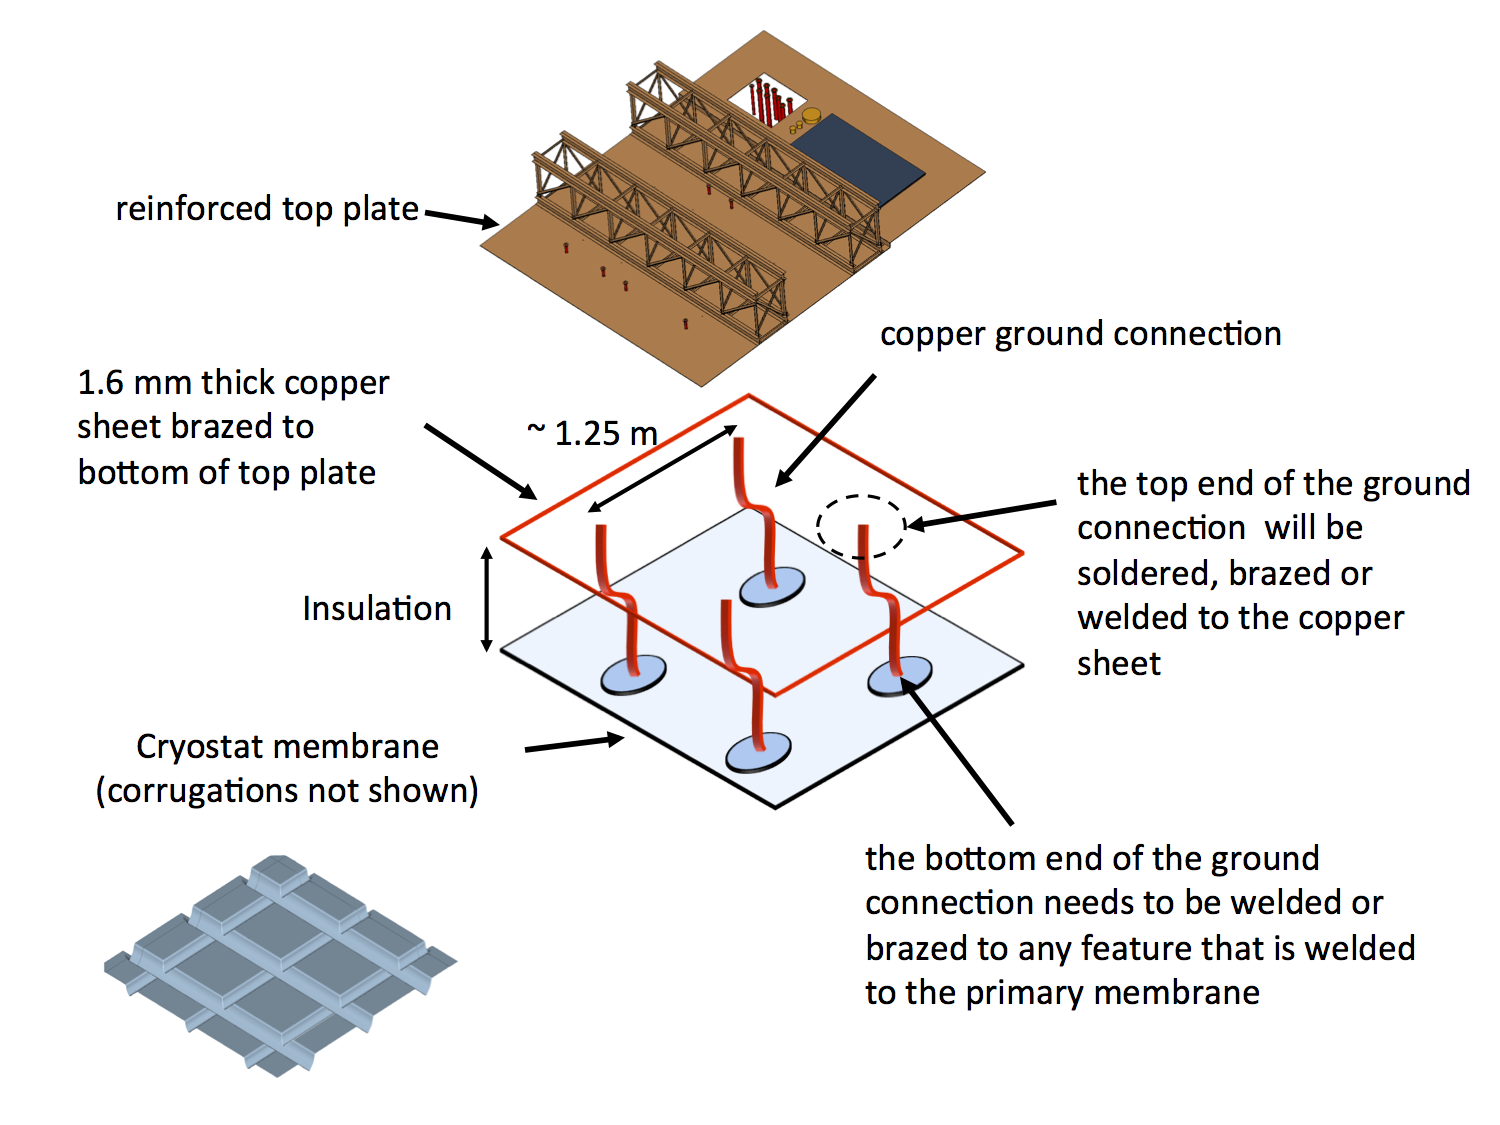
\includegraphics[width=.95\textwidth]{figures/cryostat-top-plate-gnd} % (figure 4)
\caption[Top plate grounding layout]{\label{fig:top-plate-gnd}Top plate grounding layout}
\end{center}
\end{figure}

\textbf{Leak prevention (from David Montanari)}

The primary membrane will be subjected to several leak tests and weld remediation, as necessary. All 
(100\%) of the welds will be tested by an Ammonia colorimetric leak test (ASTM E1066-95) in which 
welds are painted with a reactive yellow paint before injecting a Nitrogen-Ammonia mixture into the 
insulation space of the tank. Wherever the paint turns purple or blue, a leak is present. The developer is 
removed, the weld fixed and the test is performed another time. Any and all leaks will be repaired. The 
test lasts a minimum of 20 hours and is sensitive enough to detect defects down to 0.003 mm in size 
and to a $10^{-7} std-cm^3/s$ leak rate (equivalent leak rate at standard pressure and temperature, 1 bar and 
273 K). To prevent infiltration of water vapor or oxygen through microscopic membrane leaks (below 
detection level) the insulation spaces will be continuously purged with gaseous argon to provide one 
volume exchange per day. The insulation space will be maintained at 30 mbar, slightly above 
atmospheric pressure. This space will be monitored for changes that might indicate a leak from the 
primary membrane. Pressure control devices and safety relief valves will be installed on the insulation 
space to ensure that the pressure does not exceed the operating pressure inside the tank. The purge gas 
will be recirculated by a blower, purified, and reused as purge gas. The purge system is not safety-
critical; an outage of the purge blower would have negligible impact on LAr purity.

%%%%%%%%%%%%%%%%%
\textbf{Cryostat size from TPC dimensions  (from Jack Fowler)}

The minimum internal size of the cryostat is determined from size of the TPC.  At the bottom of the 
cryostat there needs to be a minimum of 0.3 m between the frame of the CPA and closest point on the SS 
membrane.  This is to prevent high voltage discharge between the CPA and the electrically grounded 
membrane. It is foreseen that there would be some cryogenic piping and instrumentation under the TPC.  
There is a height allowance of 0.1 m for this.  There will be access and egress space around the outside 
of the TPC and the membrane walls.  On three sides, 1.0 m of space is reserved for this.  The final side of 
the TPC will have piping and instrumentation for the cryogenic system.  There will be 1.3 m of space 
reserved for this.  

The support system for the TPC will be located at the top between the underside of the cryostat roof and 
the top of the TPC.  The plan is to model this space similar to what is planned for the far site TPC.  There 
will be 0.9 m of ullage space.  In order to prevent high voltage discharge, the upper most part of the CPA 
needs to be submerged a minimum of 0.3 m below the liquid Argon surface.  The top of the TPC will be 
separated from the membrane by a minimum of 1.2 m.  

Adding all of these to the size of the TPC yields the minimum inner dimensions of the cryostat.  A 
minimally sized cryostat would be 9.5 m long, 7.3 m wide and 8.4 m high.  This assumes the TPC will be 
positioned inside the cryostat with the CPAs and end field cages parallel to the walls of the cryostat.  Also 
there is no space allotted for a beam window to enter the cryostat.  Clearance would need to be added if 
it violates any of the current boundaries listed above.  
These dimensions also preserve the ability to reverse the order of the APAs and CPAs inside the TPC.  The 
current plan is to have the APAs located in the center of the cryostat with a CPA on each side.  Reversing 
this to have the CPA in the center and APAs on each side may be required to achieve some of the 
proposed physics.  The orientation of the TPC components will be finalized after various scenarios have 
been sufficiently simulated.  

\subsection{Cryogenic System (from David Montanari)}

The cryogenic system is being developed as part of the international engineering team set up between 
Fermilab and CERN to design, fabricate and install cryogenic systems of similar requirements and 
increased size for Short and Long Baseline at Fermilab, and WA105s at CERN. The goal is to develop a 
single model and adapt if for all future generation detectors, with the necessary scaling up in size and 
adjustments for eventual different needs of the different detectors. Table~\ref{tbl:cryo-design-parameters} presents the list of 
requirements for the cryogenic system for the Single Phase TPC test at CERN detector.

Figure~\ref{fig:proposed-LN2-system} outlines the basic scheme of the LN2 supply system, which was proposed by CERN for the Short 
Baseline Program and agreed as an appropriate solution for this detector as well. The experiment will rely 
on LN2 tankers for regular deliveries to a local dewar storage, which will be sized to provide several days 
of cooling capacity in the event of a delivery interruption. From the dewar storage the LN2 is then 
transferred to a distribution facility located in the experimental hall. It includes a small buffer volume and 
an LN2 pumping station that transfers the LN2 to the argon condenser and other services as needed. The 
low estimated heat leak of the vessel (~3.5 kW) and the location inside an above ground building allow for 
use of an open loop system typical of other installations operated at Fermilab (LAPD, LBNE 35 ton 
prototype, MicroBooNE) and at CERN (???). 
Main goal of the LN2 system is to provide cooling power for the argon condenser, the initial cool down of 
the vessel and the detector, and all other services as needed.

Figure~\ref{fig:proposed-LAr-system} shows a schematic diagram of the proposed liquid argon system. It is based on the design of the 
LBNE 35 ton prototype, the MicroBooNE detector systems and the current plans for the Long Baseline Far 
Detector.

Main goal of the LAr system is to purge the tank prior to the start of the operations (with GAr in open and 
closed loop), cool down the tank and fill it with LAr. Then continuously purify the LAr and the boil off GAr 
to maintain the required purity (electron lifetime measured by the detector).

The LAr receiving facility includes a storage dewar and an ambient vaporizer do deliver LAr and GAr to the 
cryostat. The LAr goes through the liquid argon handling and purification system, whereas the Gar through 
the gaseous argon purification before entering the vessel.
The LAr purification system is currently equipped with a filter containing mol sieve and copper beds, and a 
regeneration loop to regenerate the filter itself. The filter medium may change following the ongoing 
developments on filtration schemes, but the concept remains the same.

During operation, an external LAr pump circulates the bulk of the cryogen through the LAr purification 
system. The boil off gas is first re-condensed and then is sent to the LAr purification system before re-
entering the vessel.


\begin{table}[htpb]
\caption{Design requirements for the cryogenic system}
\label{tbl:cryo-design-parameters}
\centering
\begin{tabular}{|p{.45\textwidth}|p{.45\textwidth}|}
\hline
 \textbf{ Parameter} & \textbf{Value} \\ \hline
 Location & Preferably not in front of the cryostat (on the beam) \\ \hline
 Cooling Power & TBD based on the heat leak of the cryostat (estimated 3.5 kW), the cryo-piping and all other contributions (cryogenic pumps, etc.) \\ \hline
 Liquid argon purity in cryostat & 10 ms electron lifetime (30 ppt O2 equivalent) \\  \hline
 Gaseous argon piston purge rate of rise & 1.2 m/hr \\ \hline
 Membrane cool-down rate & From manufacturer \\  \hline
 TPCs cool-down rate & \textless40 K/hr,\textless10 K/m (vertically)
 \\ \hline
Mechanical load on TPC & The LAr or the gas pressure shall not apply a mechanical load to the TPC greater than 200 Pascal. \\ \hline
Nominal LAr purification flow rate (filling/ops) & 5.5 day/volume change \\ \hline
 Temperature of all surfaces in the ullage during operations & \textless100 K \\  \hline
 Gaseous argon purge within insulation & 1 volume change /day of the open space between insulation panels. \\ \hline
 Lifetime of the cryogenic system & Consistent with the LAr program. TBD. \\ \hline
\end{tabular}
\end{table}

\begin{figure}
\begin{center}
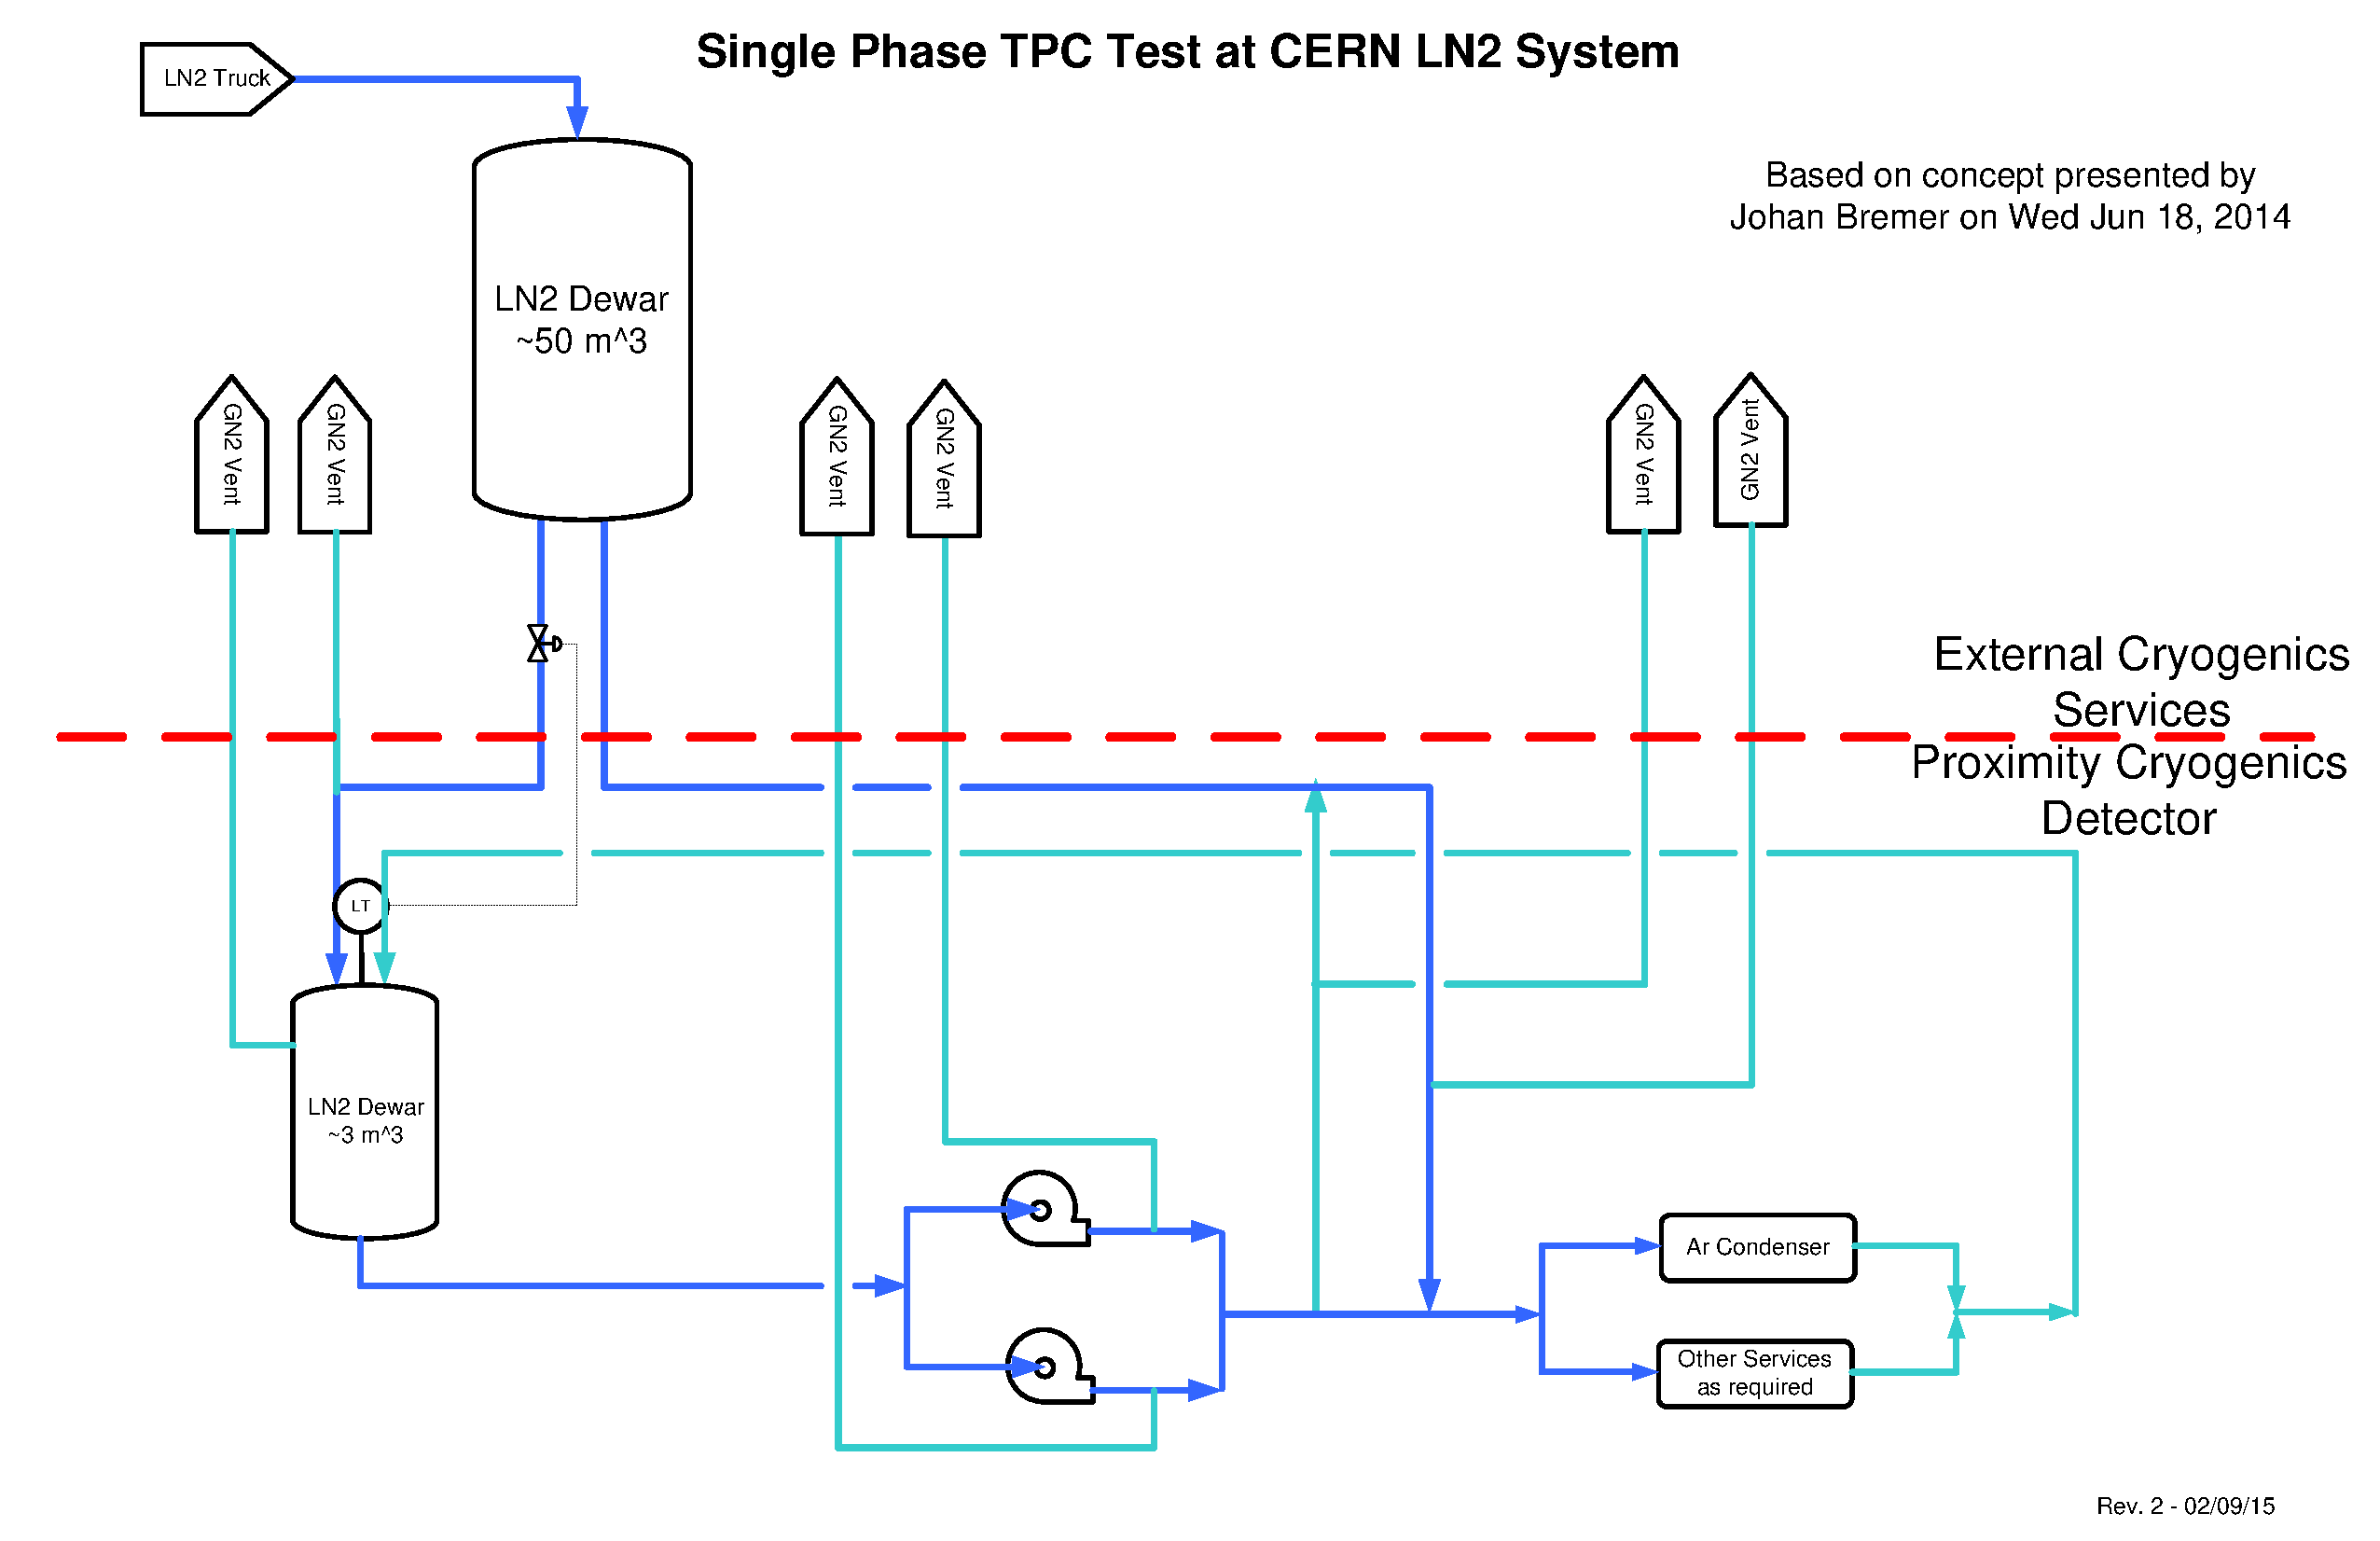
\includegraphics[width=.75\textwidth]{figures/proposed-LN2-system} % (figure 3)
\caption[Schematic diagram for the proposed LN2 system]{\label{fig:proposed-LN2-system}Schematic diagram for the proposed LN2 system}
\end{center}
\end{figure}

\begin{figure}
\begin{center}
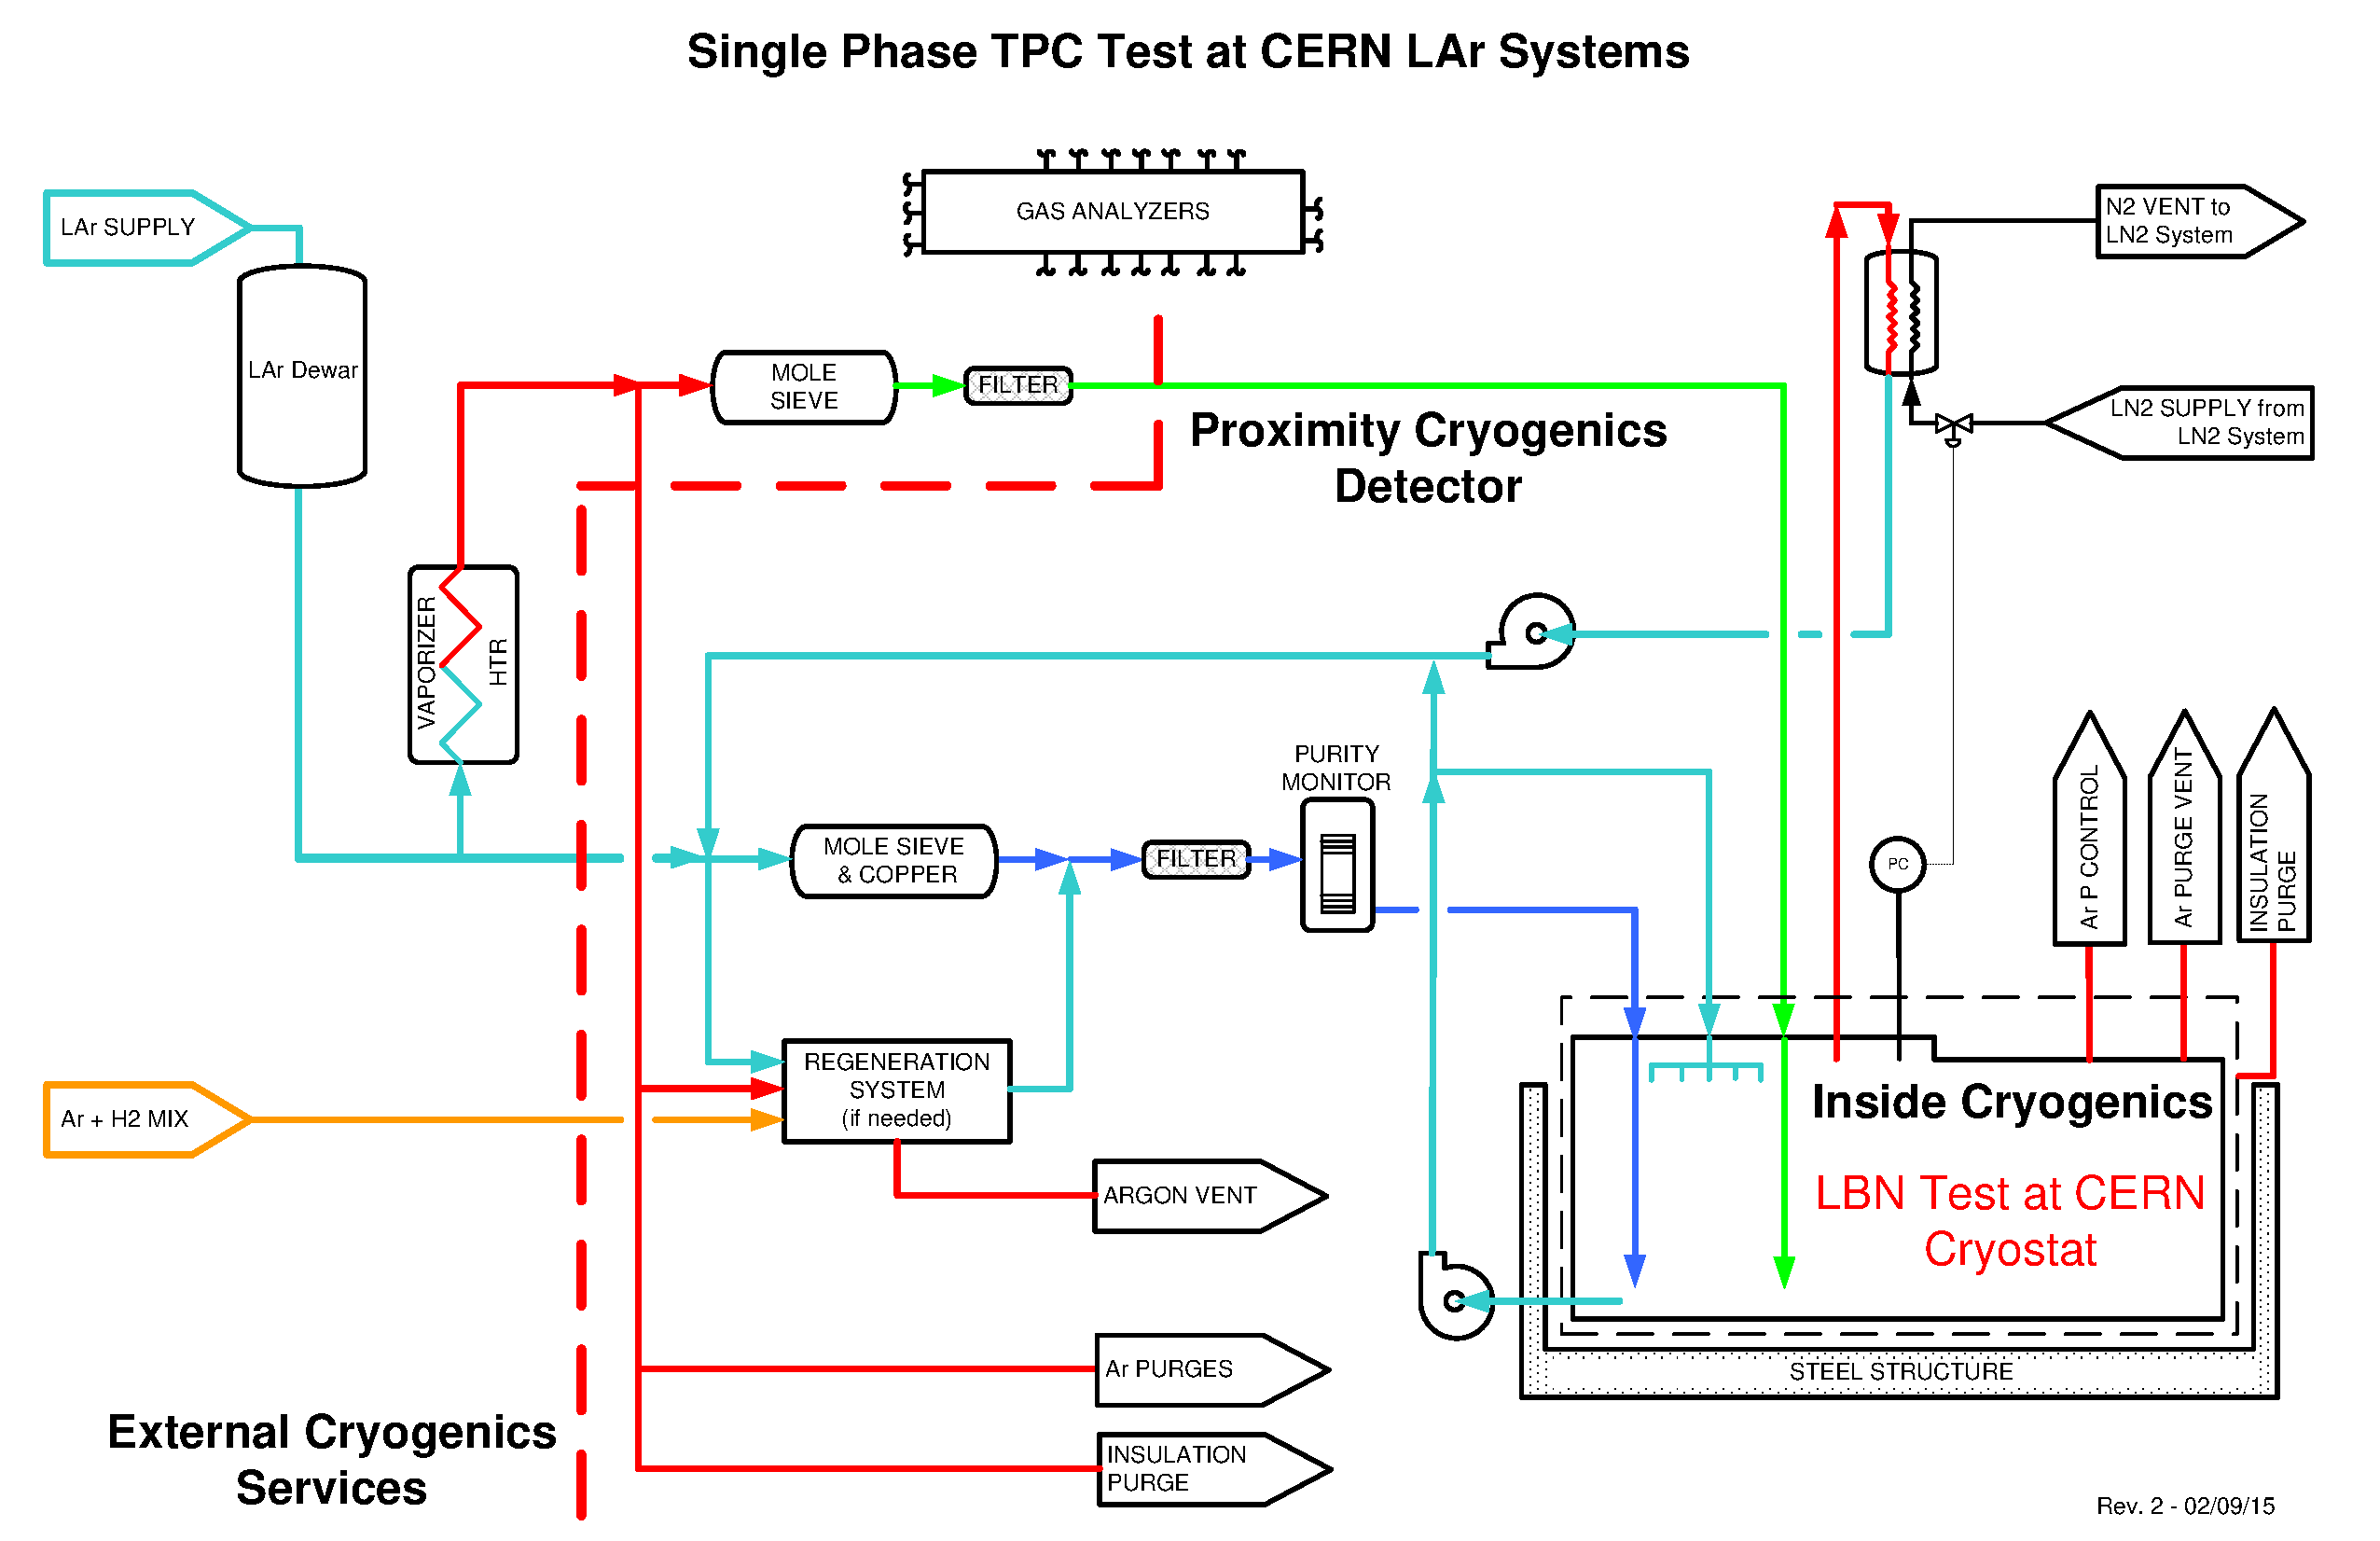
\includegraphics[width=.75\textwidth]{figures/proposed-LAr-system} % (figure 3)
\caption[Schematic diagram for the proposed LAr system]{\label{fig:proposed-LAr-system} Schematic diagram for the proposed LAr system}
\end{center}
\end{figure}


